\documentclass{patmorin}
\usepackage{amsopn,amsthm,amsmath,graphicx}
\usepackage{pat}

\DeclareMathOperator{\cn}{cr}

\newcommand{\const}{268.19}

\title{Ghost Chimneys}
\author{Barbados 2010 Gang}

\begin{document}
\maketitle

\begin{abstract}
A set $S$ of $i$ points in $\R^2$ is an $(i,t)$ set of ghost chimneys if
there exists lines $H_0,\ldots,H_{t-1}$ such the orthogonal projection
of $S$ on $H_j$ consists of exactly $i+j$ distinct points.  In this paper we give upper and lower bounds on the maximum value of $t$ in an $(i,t)$ set of ghost chimneys.
\end{abstract}

\section{Introduction}

We consider the following problem:  Given an integer $i$,
what is the maximum value $t(i)$ such that there exists a set of points
$S\subseteq\R^2$ and a set $H_0,\ldots,H_{t-1}$ of lines where, for
each $j\in\{0,\ldots,t(i)-1\}$, the orthogonal projection of $S$ onto $H_j$ consists of exactly $i+j$ distinct points.
We prove the following result:

\begin{thm}
For any integer $i$,  $ 2i -1 \le t(i) \le 124.33i$.
\end{thm}

\section{The Lower Bound}

\begin{lem}
For each integer $i\ge 1$, there exists a set $S=S(i)$ of $3i-1$
points and a set $H_0,\ldots,H_{2i-1}$ of lines such that, for each
$j\in\{0,\ldots,2i-1\}$, the orthogonal projection of $S$ onto $H_j$
has exactly $i+j$ distinct values.
\end{lem}

\begin{proof}
The point set $S$ consists of the points of a $i\times 3$ grid with the bottom-right corner removed (see \figref{lower-bound}).  For even $j$, $H_j$ is a line of slope $j/2$.  For odd $j$, $H_j$ is a line of slope $-(j+1)/2$.
\begin{figure}
  \begin{center} 
    \begin{tabular}{cc}
      & 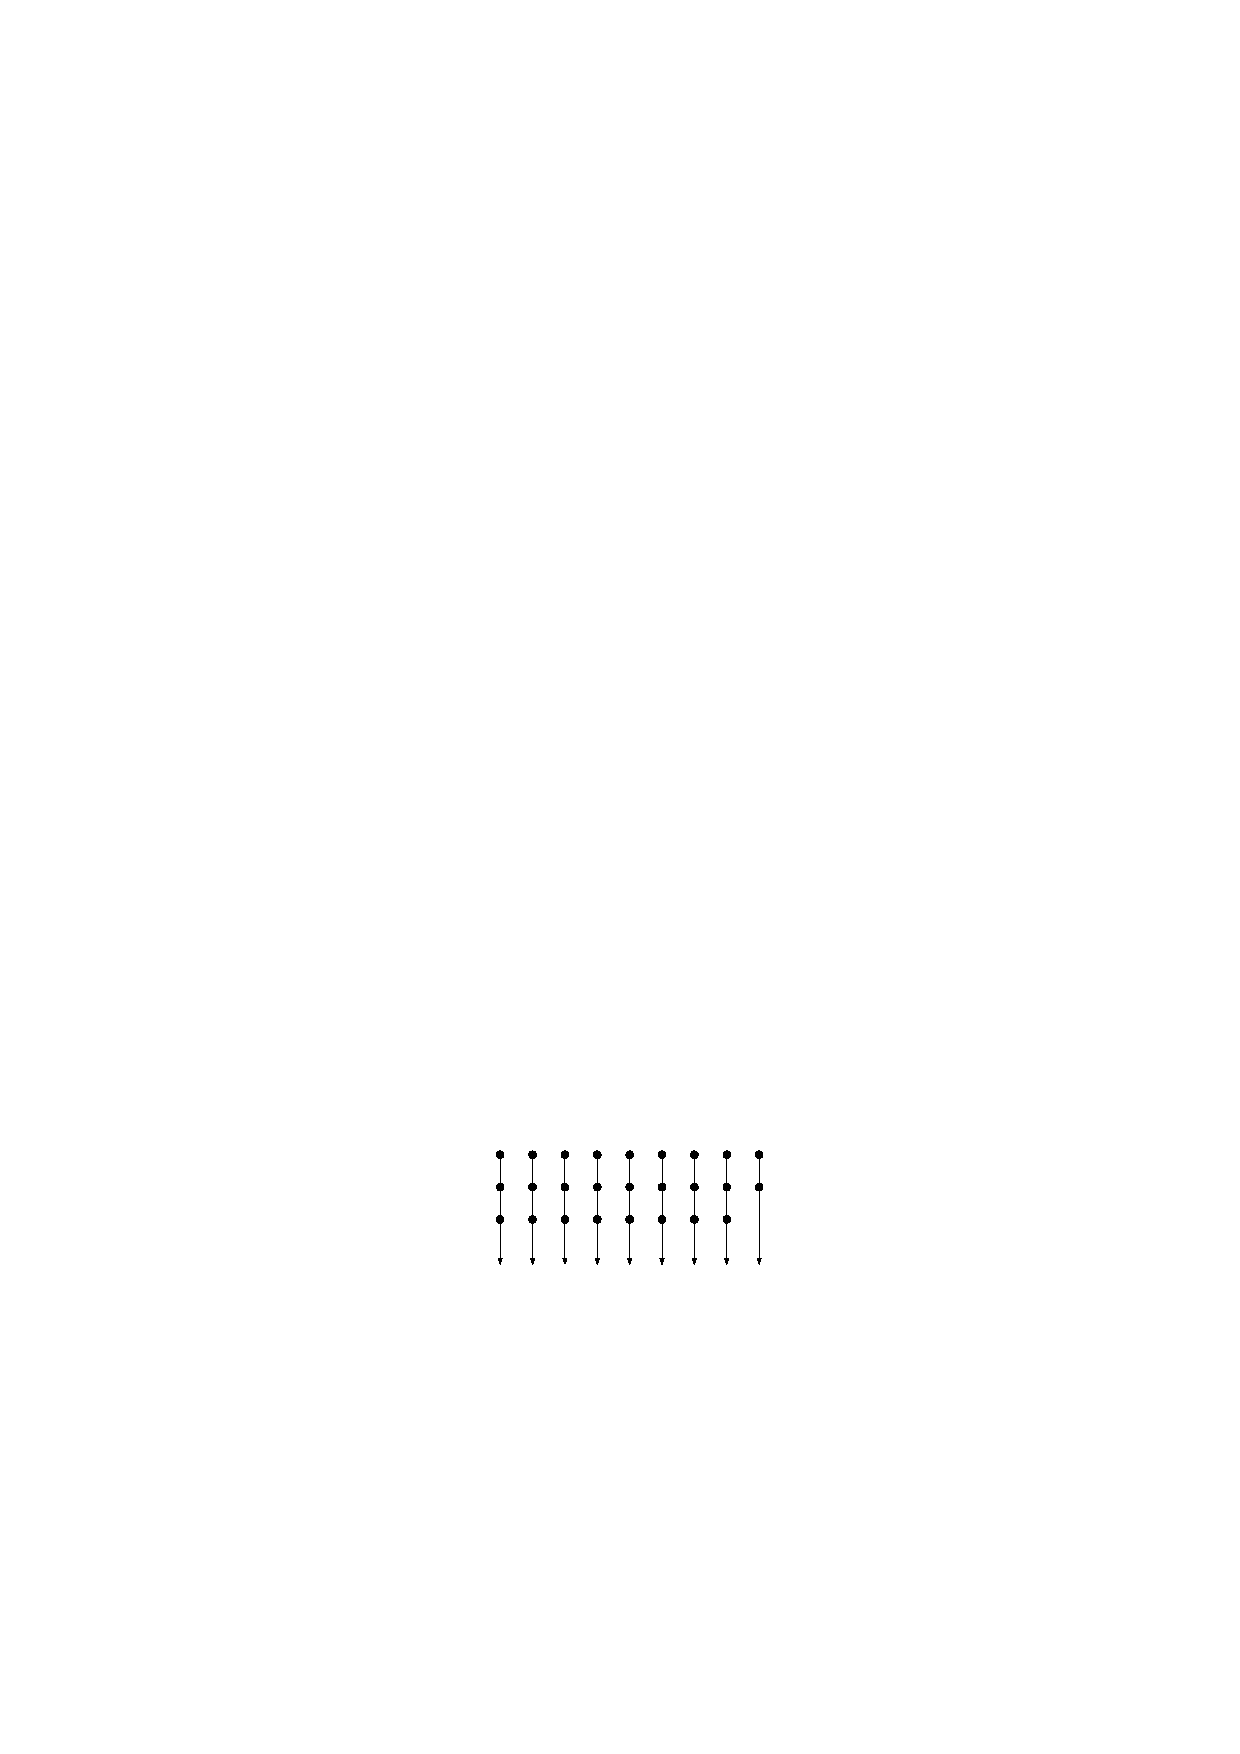
\includegraphics{j0} \\ 
      & $j = 0$  \\
       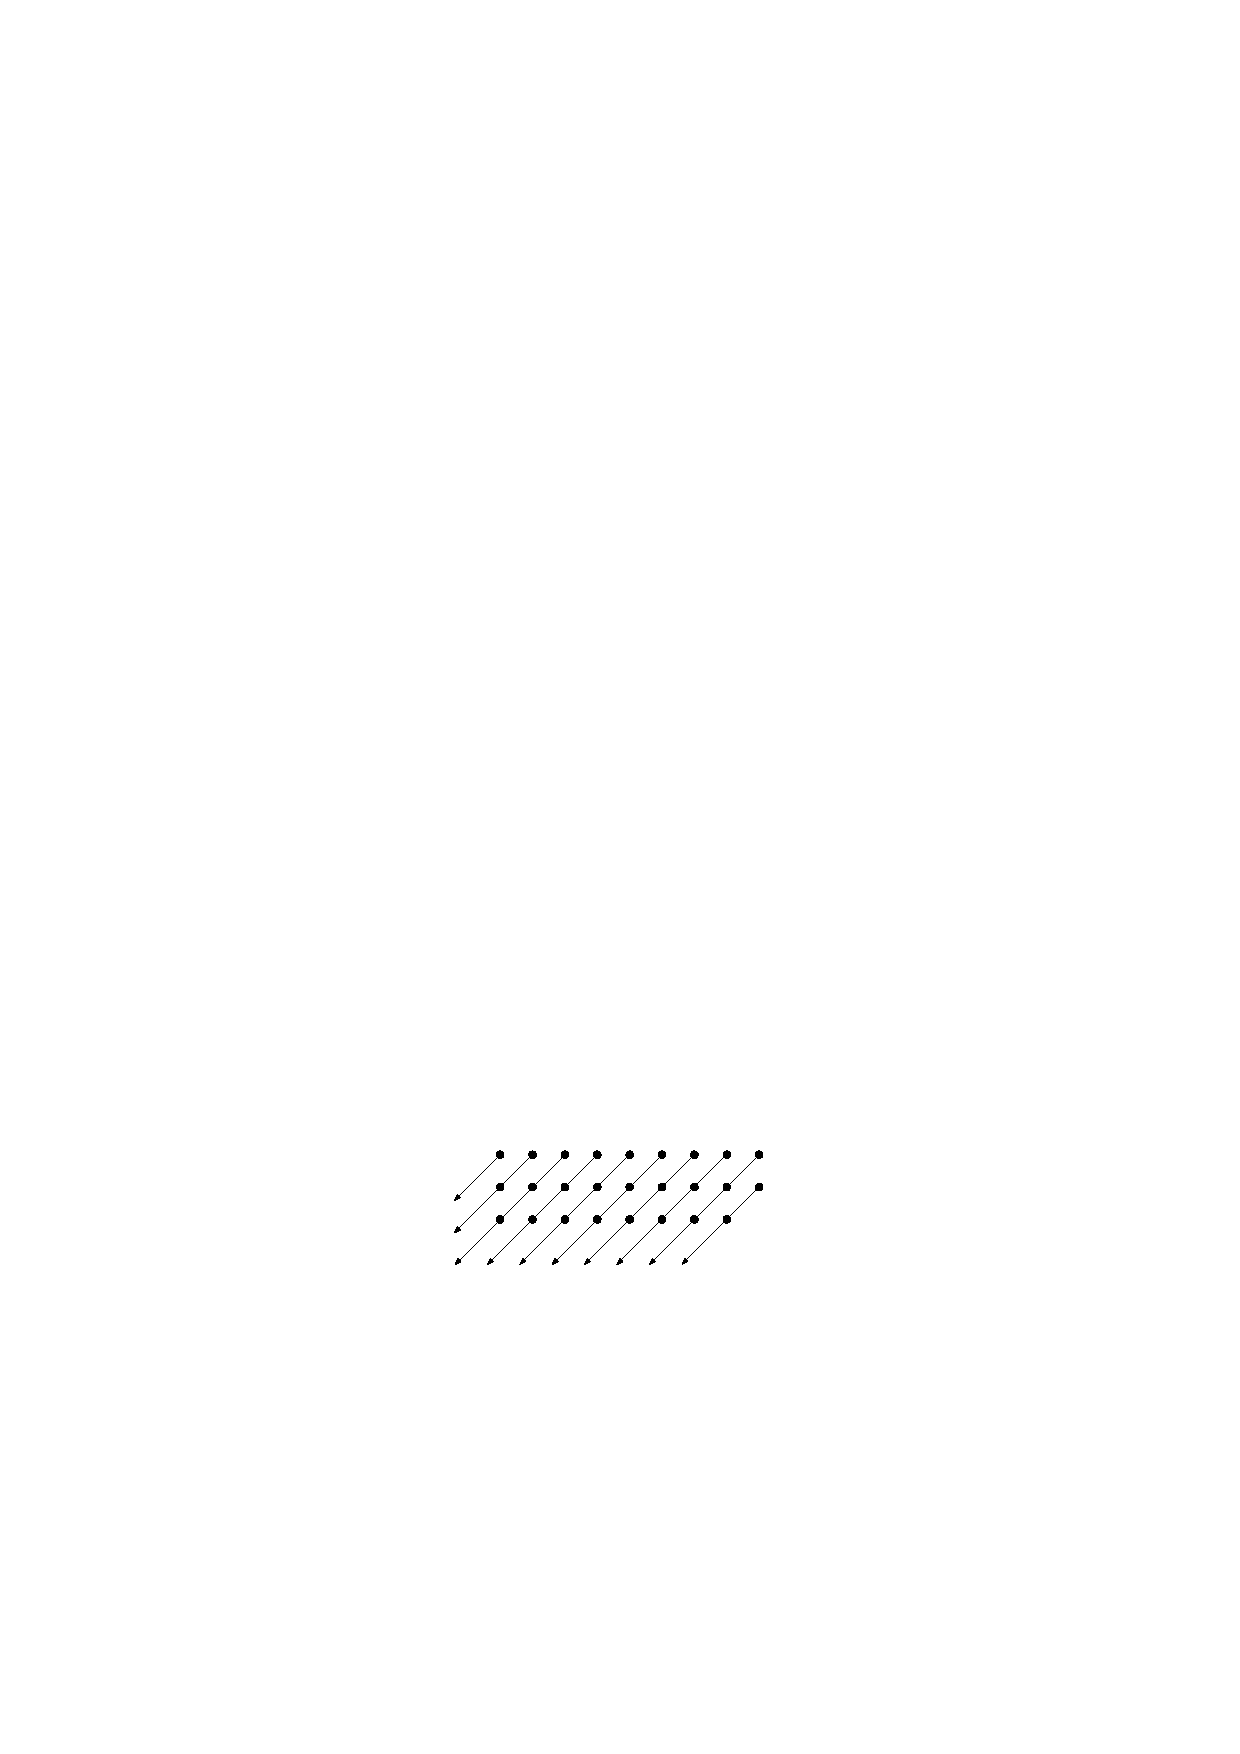
\includegraphics{j1} & 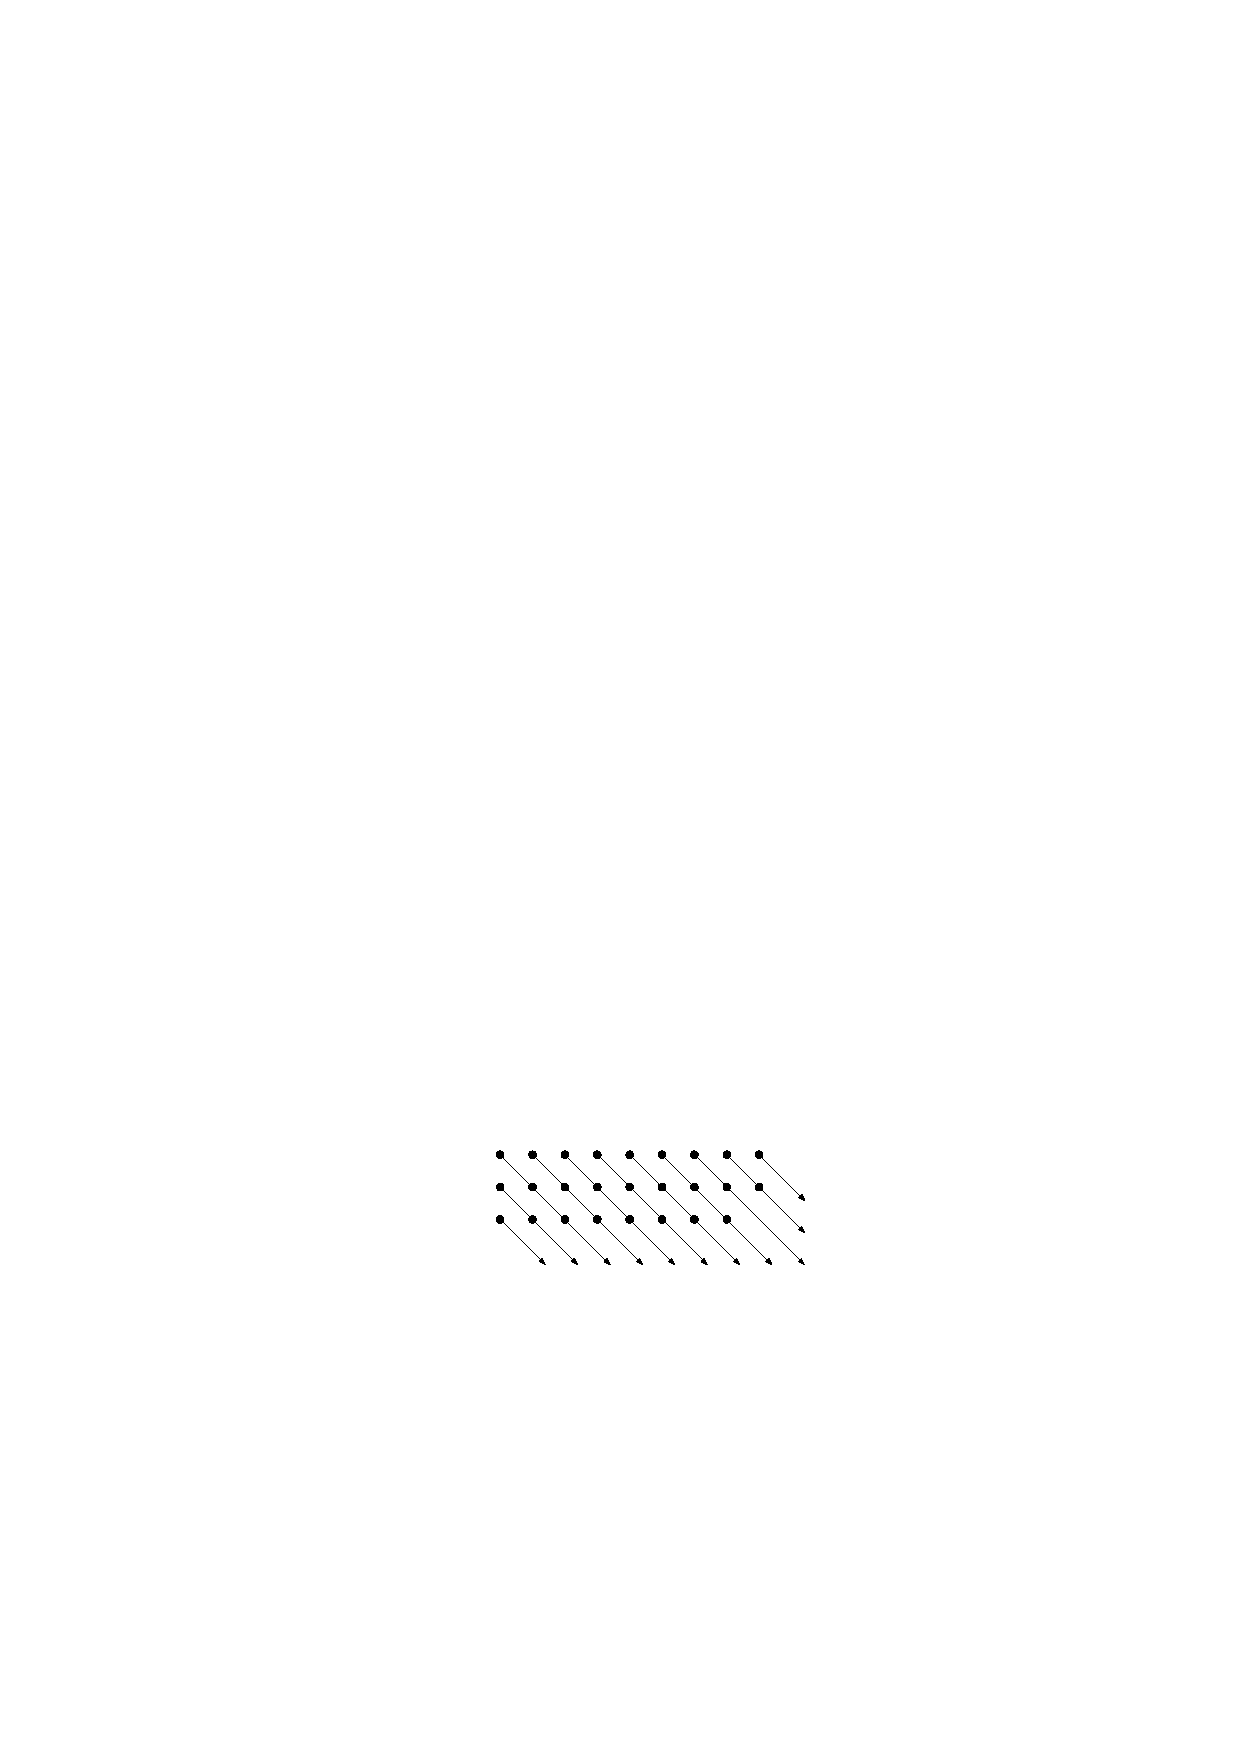
\includegraphics{j2} \\
        $j=1$ & $j=2$ \\
       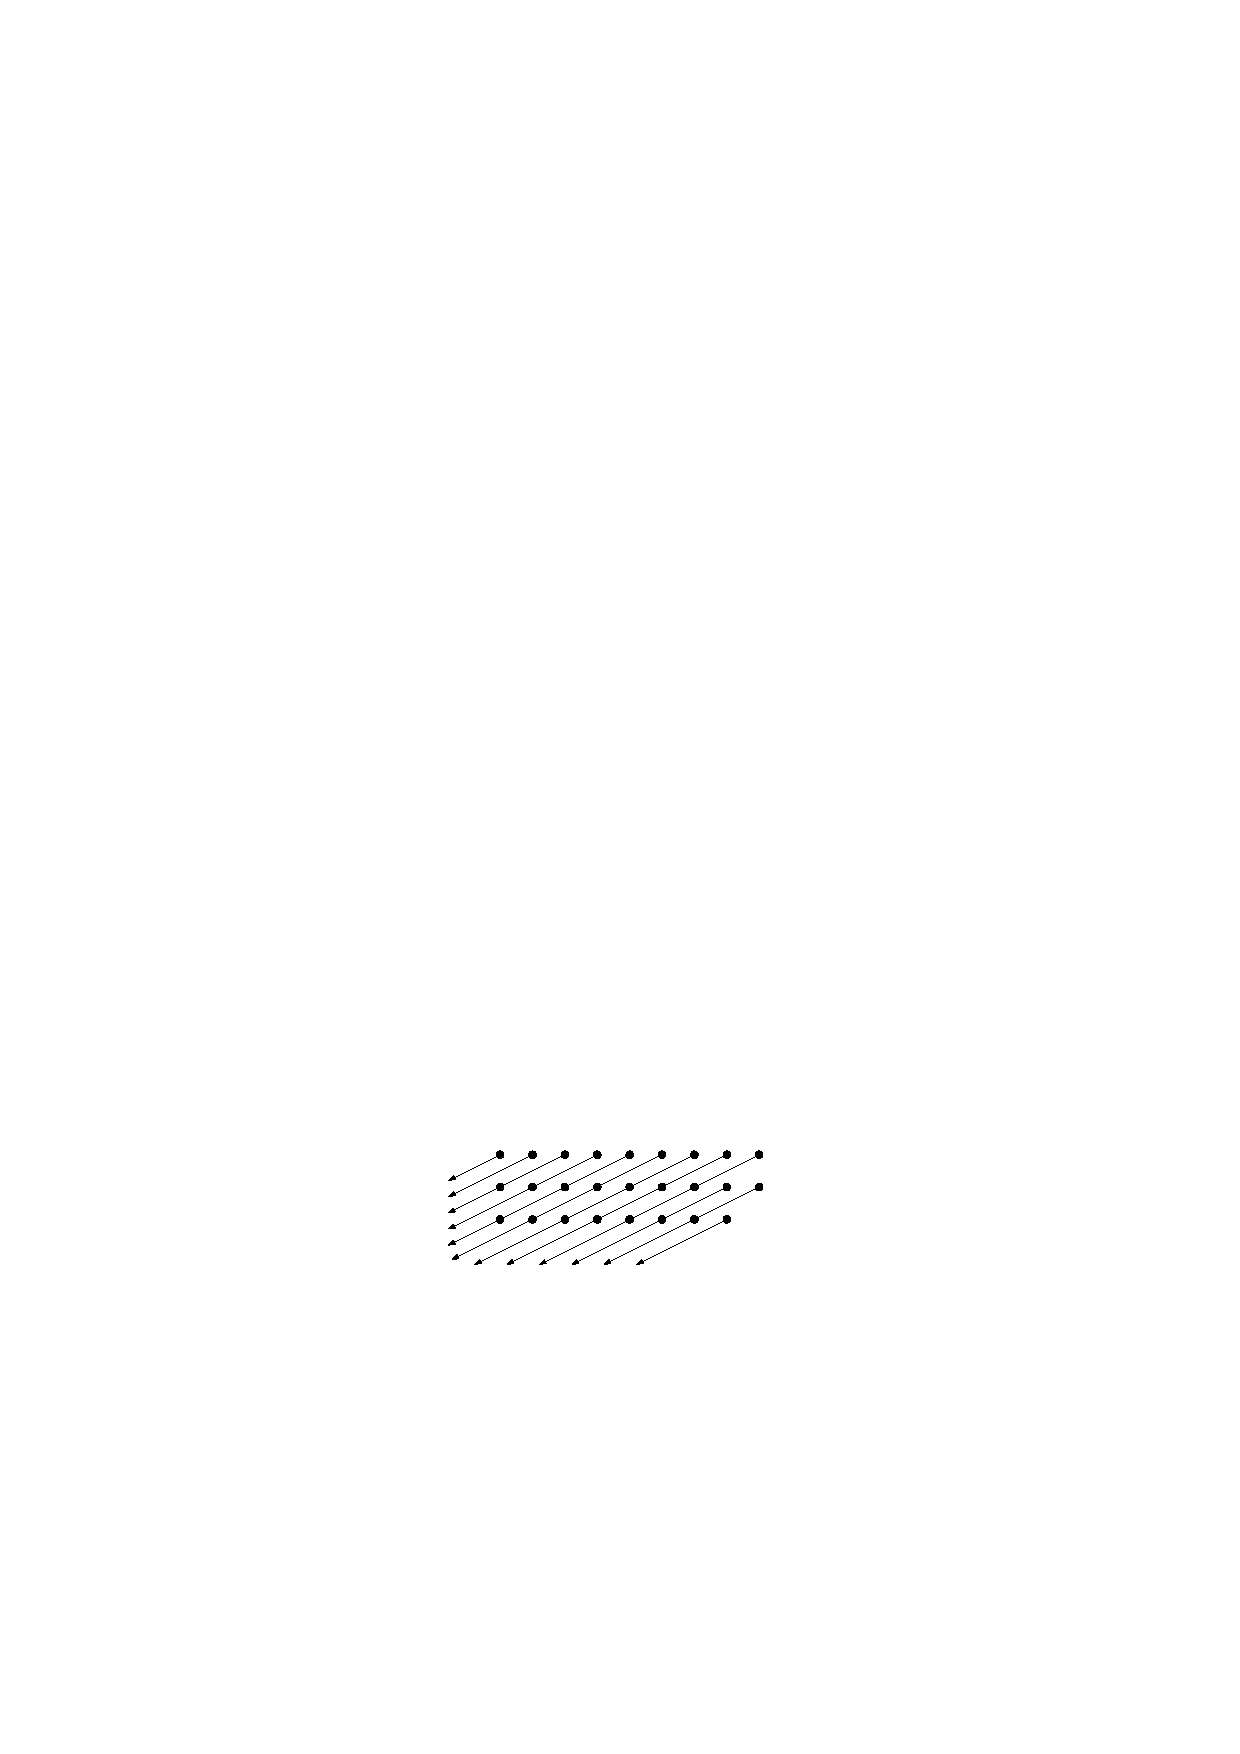
\includegraphics{j3} & 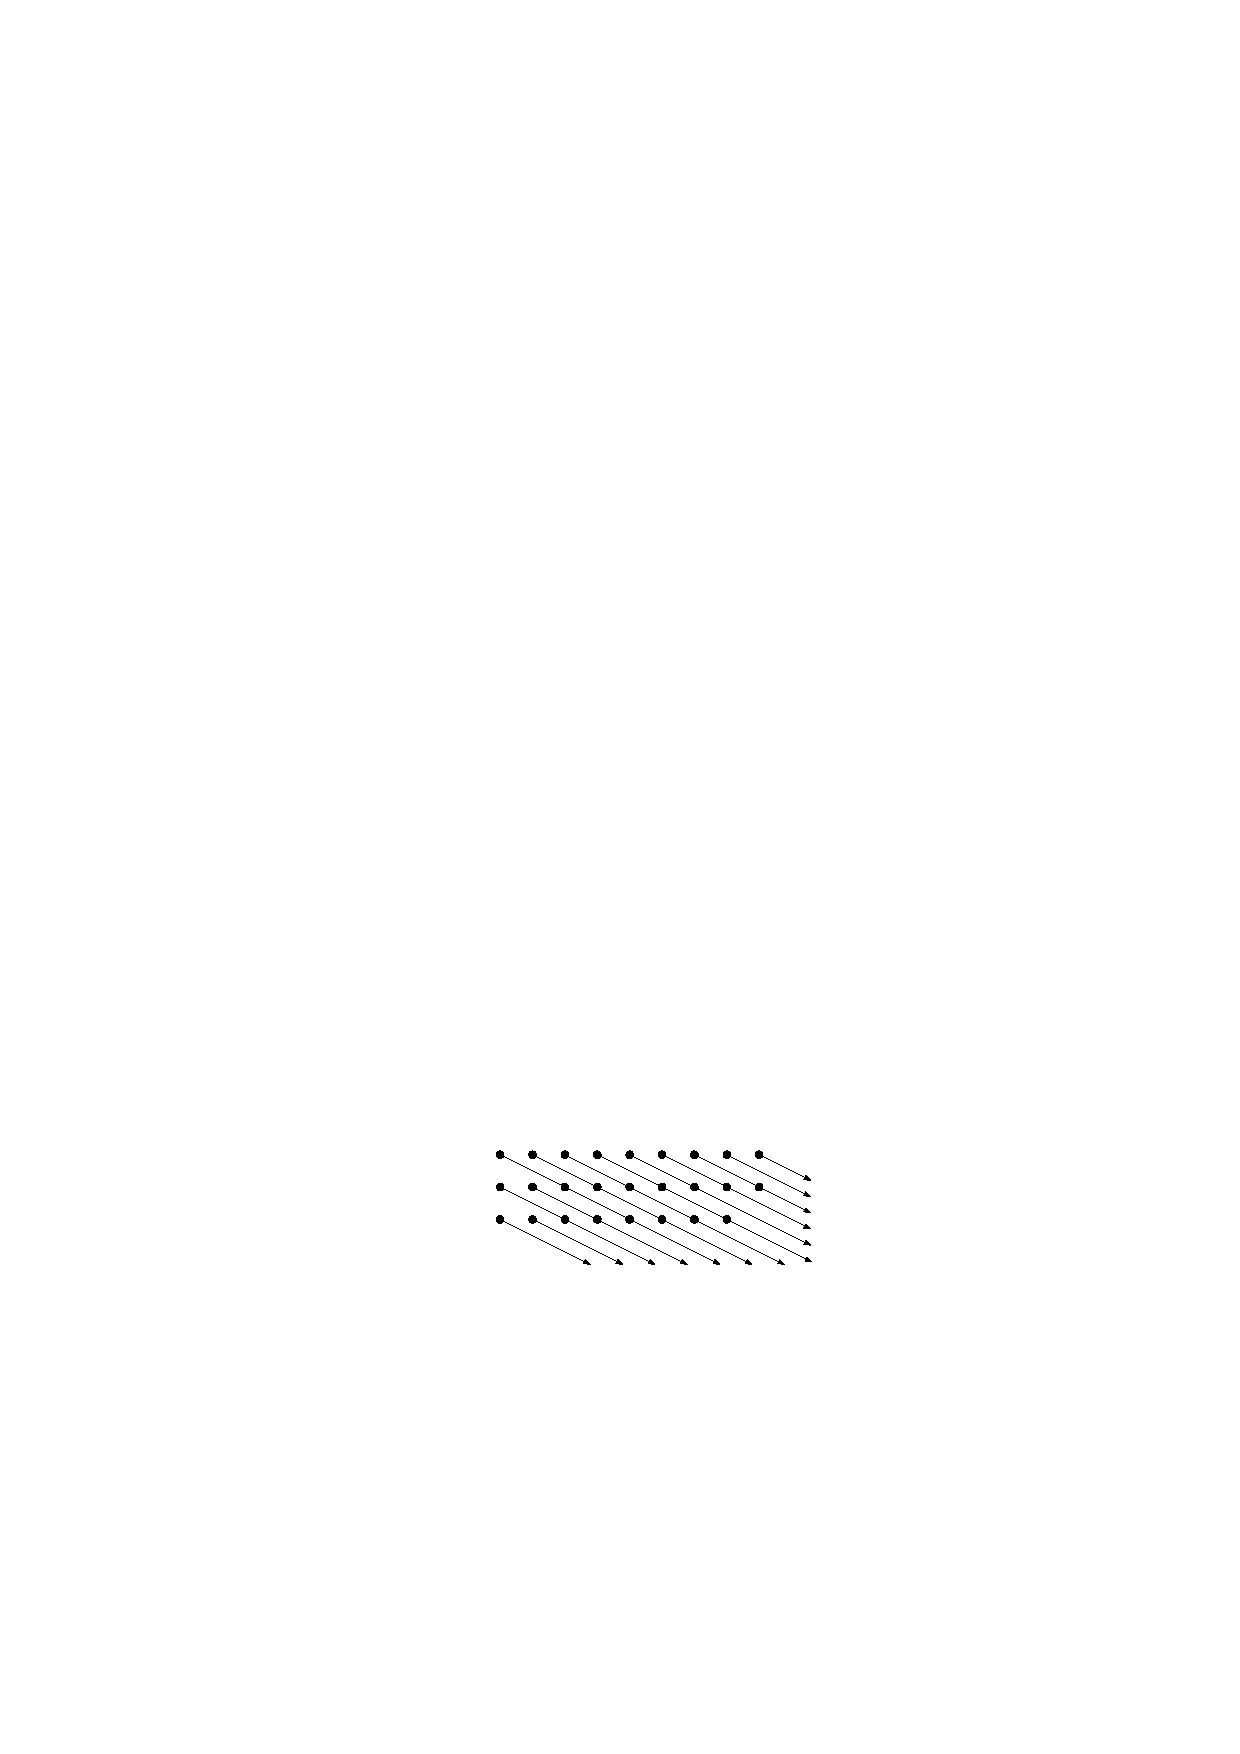
\includegraphics{j4} \\
        $j=3$ & $j=4$
    \end{tabular}
  \end{center}
  \caption{The set $S(i)$  for $i=9$ and the projection directions that yield $i,\ldots,i+4$ distinct points.}
  \figlabel{lower-bound}
\end{figure}
\end{proof}


\section{The Upper Bound}

Our upper-bound proof is closely related to Sz\'ekely's proof of the
Szem\'eredi-Trotter Theorem.  We make use of the following version of the
Crossing Lemma, which was proven by Pach, Radoici\'c, Tardos, and T\'oth
(SoCG~2004):

\begin{lem}[Crossing Lemma]\label{lem:crossing}
Let
$\beta=103/6$, $\gamma = 1024/31827$, and let
$G$ be a graph with no self loops, no parallel edges, $v$ vertices, and
$e > \beta v$ edges.  Then
\[
  \cn(G) \ge \gamma \cdot \frac{e^3}{v^2} \enspace ,
\]
\end{lem}


\begin{lem}
Let $t=\alpha i$, let $S$ be a set of $r$ points, and let
$H_0,\ldots,H_{t-1}$ be a set of lines such that the orthogonal projection
of $S$ onto $H_{j}$ gives exactly $i+j$ distinct values.  Then, $t\le 34$
or $r\le \max\{4,2/\alpha + 2 + \alpha/2\}i/\gamma$.
\end{lem}

\begin{proof}
Each projection direction $H_j$ defines a set $L_j$ of $i+j$ parallel
lines, each of which contains at least one point of $S$.  Let $G$ be the
geometric graph that contains the points in $S$ plus $t$ additional points
$p_0,\ldots,p_{t-1}$.  Two vertices in $S$ are connected by an edge in
$G$ if they occur consecutively on some line in $\bigcup_{j=0}^{t-1}L_j$.
Additionally, each vertex $p_j$ is connected the $i+j$ extreme points
on the lines in $L_j$.  See \figref{graph}.

The graph $G$ has $t+r$ vertices
and $tr$ edges.  Observe that we have a drawing of $G$ so that the only
crossings between edges occur where lines in $L$ intersect each other.
The total number of intersecting pairs of lines in $L$ is
\[
  \begin{aligned}
    X(G) 
      & = \sum_{j=1}^{t-1}(i+j)\cdot\sum_{k=0}^{j-1}(i+k) \\
      & \le \sum_{j=1}^{t-1}(i+j)(ij + j^2/2) \\
      & \le \sum_{j=1}^{t-1}(i^2j+3ij^2/2 + j^3/2) \\
      & \le i^2t^2/2 + it^3/2 + t^4/8 \enspace .
  \end{aligned}
\]

Applying \lemref{crossing}, we obtain learn that either
\begin{equation}
   tr \le \beta (t+r) \enspace , \eqlabel{crossing-a}
\end{equation}
or
\begin{equation}
   X(G) \ge \cn(G) \ge \gamma \frac{(tr)^3}{(t+r)^2} \eqlabel{crossing-b} \enspace .
\end{equation}

In the former case, we rewrite \eqref{crossing-a} to obtain
\[
   t \le \beta(t/r + 1) \le 2\beta \le 34 + 1/3 \enspace ,
\]
so $t\le 34$ (since $t$ is an integer).

In the latter case, we rewrite \eqref{crossing-b} to obtain
\[ i^2t^2/2 + it^3/2 + t^4/8 \ge \gamma\frac{(tr)^3}{(t+r)^2} .  \]
Substituting $t=\alpha i$ gives
\[ i\left(\frac{1}{2\alpha} 
    + \frac{1}{2}+\frac{\alpha}{8}\right) 
      \ge \gamma \frac{r^3}{(t+r)^2} \ge \gamma r/ 4 \enspace ,
\]
where the second inequality follows from the fact that $t \le r$.  Rewriting to isolate $r$ finally gives
\[
  r \le \left(\frac{2}{\alpha} + 2 +\frac{\alpha}{2}\right)i/\gamma \enspace .
\]
We finish the proof by observing that, for $\alpha > 2$, the inequality $r\le 4i/\gamma$ obtained by setting $\alpha=2$ is stronger and still applies.
%
%
%Next we observe that the number of points, $r$, satisfies
%\[  r \ge i+t-1 
%\]
%since there are $i+t-1$ parallel lines in $L_{t-1}$ and each of these
%contains at least one point of $S$.  Furthermore, the points of $S$
%are all contained in the intersections of lines in $L_{i}$ with lines
%in $L_{i+1}$, so
%\[
%   r \le i(i+1) \enspace .
%\]
%
%Define a geometric graph $G$ whose vertices are the points in $S$ and
%in which two points are connected if they occur consecutively on some
%line $L_j$. Observe that $G$ is a graph with no self-loops and no
%parallel edges. The number of
%edges in $G$ is exactly $tr - \ell(t)$.
%
%At this point, one would normally apply the Crossing Lemma
%(Lemma~\ref{lem:crossing}) to $G$.  However, this turns out to be
%insufficient to prove a linear bound on $t$.  Instead, we will consider
%a subgraph of $G$.  Let $G_{s}$, $s\in\{1,\ldots,t\}$, be defined like
%$G$, but only with respect to the set of lines in $L_0,\ldots,L_{s-1}$.
%Then, by Lemma~\ref{lem:crossing},
%\begin{equation}
%   sr - \ell(s) \le \beta r
%     \label{eq:few-edges}
%\end{equation}
%or
%\begin{equation}
%  \chi(s) \ge \gamma\cdot\frac{(sr-\ell(s))^3}{r^2}
%     \label{eq:many-crossings}
%\end{equation}
%for each $s\in\{0,\ldots,t-1\}$.
%In particular, select $s=2i$.  Then Eq.~(\ref{eq:few-edges}) implies that
%\[  
%   2ir - \ell(2i)  \le \beta r
%\]
%which implies that $r \le \ell(2i)/(2i-\beta)$, so 
%STOPPED HERE
%\[
%  t < 2/(2i/\beta-1) - \ell(s)/\beta - i + 1 \le \const i + 1
%\]
%for every non-negative integer $i$.
%Therefore, we may assume that 
%Eq.~(\ref{eq:many-crossings}) holds.
%Letting $t=ci$ and 
%rewriting Eq.~(\ref{eq:many-crossings}), we get
%\[
%  \begin{aligned}
%  s 
%   &\le \frac{\chi(s)^{1/3} (r+2)^{2/3}}{\gamma^{1/3}r} 
%       - \frac{\ell(s)}{r} \\ 
%   &\le \frac{\chi(s)^{1/3} (r^{2/3}+2^{2/3})}{\gamma^{1/3}r} 
%      - \frac{\ell(s)}{r} \\
%   & = \frac{\chi(s)^{1/3}r^{2/3}+\chi(s)^{1/3}2^{2/3}}{\gamma^{1/3} r} 
%          - \frac{\ell(s)}{r}  \\
%   & = \frac{\chi(s)^{1/3}r^{2/3}}{\gamma^{1/3} r} 
%           +\frac{\gamma^{-1/3}(2\ell(s))^{2/3} - \ell(s)}{r} 
%    & \mbox{ (since $\chi(s) \le \ell(s)^2$)} \\
%   &\le \frac{\chi(s)^{1/3}}{(\gamma r)^{1/3}}
%    & \mbox{ (for $\ell(s) \ge 125 \Leftrightarrow i\ge 8$))} \\
%   &\le \frac{(i^2s^2/2 + is^3/2 + s^4/8)^{1/3}}{(\gamma r)^{1/3} }  \\
%   &\le \frac{((is)^{2/3}/2^{1/3} + i^{1/3}s/2^{1/3} + s^{4/3}/2)}{(\gamma r)^{1/3}}  \\
%   &\le \frac{(2^{1/3}+2^{2/3}+2^{1/3})i^{4/3}}{(\gamma r)^{1/3}}  
%    & \mbox{ (since $s=2i$)} \\
%   & = \frac{(2^{4/3} + 2^{2/3})i^{4/3}}{(\gamma r)^{1/3}}  \\
%   & =  \frac{(2^{4/3} + 2^{2/3})i^{4/3}}{(\gamma(i+t-1))^{1/3}} \\ 
%   &\le  \frac{(2^{4/3} + 2^{2/3})i^{4/3}}{(\gamma(1+c-1/i)i)^{1/3}}  
%    & \mbox{ (since $t=ci$)} \\
%   & =  \frac{(2^{4/3} + 2^{2/3})i}{(\gamma(1+c-1/i))^{1/3}} \\ 
%   & < 2i = s
%  \end{aligned}
%\]
%where the last inequality yields the desired contradiction provided that
%$c > (2^{1/3} + 2^{-1/3})^3/\gamma-1+1/i$.  Selecting $c=\const+1/i$
%gives $t=\const i + 1$ and completes the proof.
\end{proof}



\end{document}
